
\documentclass{minimal}
\usepackage{tikz}
\usepackage{tikz-qtree}

\begin{document}

\usetikzlibrary{trees, arrows, shapes.multipart}
\definecolor{pf7}{RGB}{166, 118, 29}
\tikzset{
  edge from parent/.style={draw,-latex},
  level distance=1.5cm
}
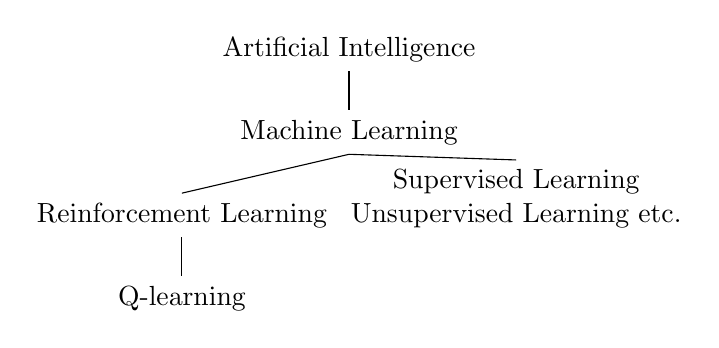
\begin{tikzpicture}[
    every node/.style={align=center,anchor=north},
  ]
  \Tree [.{Artificial Intelligence}
    [.{Machine Learning}
      [.{Reinforcement Learning}
	[.{Q-learning} ]
      ]
      [.{Supervised Learning \\ Unsupervised Learning etc.} ]
    ]
  ]
\end{tikzpicture}

\end{document}
